\documentclass[preprint,11pt,3p]{article}

\usepackage{tocloft}
\usepackage{color}
\usepackage{hyperref}
\usepackage{graphicx}
\usepackage{float}
\usepackage{subcaption}
\usepackage{amsmath} 
\usepackage{tikz} 
\usepackage{epigraph}
\usepackage{lipsum} 
\usepackage{indentfirst}
\usepackage[strings]{underscore}


\renewcommand\epigraphflush{flushright}
\renewcommand\epigraphsize{\normalsize}
\setlength\epigraphwidth{0.7\textwidth}
\renewcommand{\abstractname}{Executive Summary}

\definecolor{titlepagecolor}{cmyk}{1,.60,0,.40}

\DeclareFixedFont{\titlefont}{T1}{ppl}{b}{it}{0.5in}

\makeatletter                       
\def\printauthor{%                  
    {\large \@author}}              
\makeatother
\author{%
    Eric Altenburg \\
    \texttt{ealtenbu@stevens.edu}\vspace{20pt} \\
    Michael McCreesh \\
    \texttt{mmccree1@stevens.edu}\vspace{20pt} \\
    Hamzah Nizami \\
    \texttt{hnizami1@stevens.edu}\vspace{20pt} \\
    Constance Xu \\
    \texttt{cxu16@stevens.edu}
    }

% The following code is borrowed from: https://tex.stackexchange.com/a/86310/10898

\newcommand\titlepagedecoration{%
\begin{tikzpicture}[remember picture,overlay,shorten >= -10pt]

\coordinate (aux1) at ([yshift=-15pt]current page.north east);
\coordinate (aux2) at ([yshift=-410pt]current page.north east);
\coordinate (aux3) at ([xshift=-4.5cm]current page.north east);
\coordinate (aux4) at ([yshift=-150pt]current page.north east);

\begin{scope}[titlepagecolor!40,line width=12pt,rounded corners=12pt]
\draw
  (aux1) -- coordinate (a)
  ++(225:5) --
  ++(-45:5.1) coordinate (b);
\draw[shorten <= -10pt]
  (aux3) --
  (a) --
  (aux1);
\draw[opacity=0.6,titlepagecolor,shorten <= -10pt]
  (b) --
  ++(225:2.2) --
  ++(-45:2.2);
\end{scope}
\draw[titlepagecolor,line width=8pt,rounded corners=8pt,shorten <= -10pt]
  (aux4) --
  ++(225:0.8) --
  ++(-45:0.8);
\begin{scope}[titlepagecolor!70,line width=6pt,rounded corners=8pt]
\draw[shorten <= -10pt]
  (aux2) --
  ++(225:3) coordinate[pos=0.45] (c) --
  ++(-45:3.1);
\draw
  (aux2) --
  (c) --
  ++(135:2.5) --
  ++(45:2.5) --
  ++(-45:2.5) coordinate[pos=0.3] (d);   
\draw 
  (d) -- +(45:1);
\end{scope}
\end{tikzpicture}%
}

\begin{document}
\begin{titlepage}

\noindent
\titlefont Cruise Control Software Development Version 0.10\par
\epigraph{We pledge our honor that we have abided by the Stevens Honor System.}%
{\textit{CS347: Software Development Processes |  Spring 2020}\\ \textsc{Team Mike}}
\null\vfill
\vspace*{1cm}
\noindent
\hfill
\begin{minipage}{0.35\linewidth}
    \begin{flushright}
        \printauthor
    \end{flushright}
\end{minipage}
%
\begin{minipage}{0.02\linewidth}
    \rule{1pt}{125pt}
\end{minipage}
\titlepagedecoration
\end{titlepage}




\newpage

\tableofcontents
\newpage

\section{Executive Summary}
Team Mike is a startup initiative aimed at solving problems that come to light as
society begins to adopt new technologies. One of which pertains to autonomous
driving and “smart cars” as they are beginning to break into the automobile
market more and more every year with examples such as Tesla and Ford. In a
perfect world, if every driving car were to be a smart car with “autopilot,” then
it would make sense for each of them to communicate cruise control data with
each other to reduce traffic build-up and make traveling more efficient. Through
rotational leadership on a monthly basis, each team member possesses a set of
distinct skills that can translate to highly efficient work sessions. Aside from
developing a traditional cruise control, the aim is to make the software open source as it will serve as the foundation to a more interconnected logistical future in which autonomous cars can fully achieve
their potential within a growing technologically advanced society. 
\newpage

\section {Introduction}
The past century has seen an explosion of innovation on a scale never before seen
in human history. The rapid development and refinement of a myriad of motor
technologies catalyzed the innovation process by allowing ideas to transfer at
rates never before seen. With the constraint of distance loosening thanks to
every iteration of the automobile, people have been granted more freedom to
do what they please. While the automobile has enhanced society in several
ways, there are some glaring problems that need to be addressed to continue
the current rate of human progress and innovation. One of the biggest problems
is driver fatigue, which is responsible for approximately 72,000 crashes annually.
Programming the automobile to be reliably autonomous to a degree is one way
to circumvent the issue of driver fatigue and making roads safer. That’s exactly
what cruise control aims to do. By moderating the speed of the vehicle by itself,
cruise controls aim to lessen the effects of driver fatigue on the road. However,
the technology is not perfect, and Team Mike aims to resolve that by creating
the perfect cruise control system. \par
When it was implemented in 1958, cruise control was suitable for that era,
however, as technology continually improves, the embedded software must as
well. For longer car trips, it does not make sense for users to constantly accelerate
and decelerate for several miles; this is where cruise control comes in. By being
able to set the speed, the user is now able to accurately set and maintain the
speed they wish to without having to constantly intervene which, over time,
would cause less harm to the vehicle as variable speed and RPMs are not as
desirable as that of near-constant. \par
Our group intends to use an Agile method to implement our version of cruise
control. This would encourage code sprints in two-week lengths where work
will be divided into smaller sections and distributed based on each members’
strengths. The Agile method may vary as to which one we specifically choose
but regardless, this project will not come to fruition using Waterfall or other
methods. The way that we are going to organize our group is through weekly
meetings and ensuring that everyone knows their tasks for the week. These
weekly meetings can also serve as a place where team members mention any
obstacles that have come in their way when trying to resolve a problem, and
also serve as a time where the team as a collective can try to think of solutions
around those obstacles. We also plan on giving real-time updates about any
progress made through Slack in order to ensure all members of the team are
equipped with the most recent developments of the project. We also intend on
using Java to implement our cruise control system. We believe that the
high-performance Java provides and the fact that its part of the Object-Oriented
Programming (OOP) paradigm makes it perfect for embedded systems. \par
There are a plethora of features that make up cruise control. As most cruise
controls are seen on vehicles, there are generally a few buttons: increase speed
(and sometimes decrease speed) and the button that starts cruise control. Once
cruise control is set, the user then has the ability to increase, decrease, or
maintain the speed of a vehicle. Furthermore, if the user presses on the brake,
then cruise control is automatically deactivated. The system also allows for the
operator of a vehicle to manually deactivate it. \par
To successfully implement the features of maintaining a steady speed and a
safe distance away from other cars, there are certain requirements to fulfill. At a
high level, proper hardware with fast, reliable sensors is critical for this project.
Furthermore, lives are fundamentally dependent on this product and therefore
it requires software that is error-resistant and thus a strong development and
QA (quality assurance) team. In addition, the software must also perform it’s
expected tasks of moderating speed, maintaining a safe distance and switching
back control to the driver when prompted to quickly. Having a cruise control
software that is slow would be ineffective, so speed and accuracy are critical
requirements for the software as well as the hardware. This is a mission-critical
system because if it were to fail, it would put the lives of people in danger.

\newpage
\section{Requirements}

\subsection{Input}
\begin{enumerate}
	\item The system shall accept electric power from the alternator.
	\item The power button that allows for the state of the system to change from on to off or vice versa.
	\item When pressed, a button will either accelerate or decelerate in 1 mph increments. 
	\item When the brake is pressed, the cruise control system will unset the speed and give control back to the user until the user specifies a new speed to be set.
	\item If the entire car turns off, then a signal will be sent to turn off the cruise control system.
	\item RPM (Rotations Per Minute) sensor should be connected to the front axle and able to take readings for accurate speed calculations. 
	% \item RADAR sensor must be able to detect nearby vehicles/obstacles to avoid collision. %Do we really wanna do this
	\item Engine sensor must be able to take input from the engine to tell the cruise control system to turn on or off.
		\begin{enumerate}
			\item If the engine is turned on, the cruise control system must be ready for use within 3 seconds of the engine being turned on.
		\end{enumerate}
	\item If the gas pedal is pressed, the vehicle will continue to accelerate at the control of the user, but when the gas pedal is released the cruise control system will continue to the previously set speed.
	% \item Brake pedal sensor must be able to take input from user to stop when pressed and keep going when released.
\end{enumerate}

\subsection{Output}
\begin{enumerate}
	\item Keep a log of activity in the system files to help debug in the event of a malfunction.
	\item For every speed increase made by the user in the cruise control system, a visual indication by the software is necessary. This is so that the user minimizes their own human error. So, every time you increase the speed, you can see the cruise control speed on the car menu increasing by however much the user wants it to.
	\item The system displays successful activation or deactivation in 10 milliseconds. 
		\begin{enumerate}
			\item Numbers are subject to change depending on how inputs are received from surrounding system, but are expected to be in around that same ballpark.
		\end{enumerate}
	\item Keep a log of every time the cruise control system is used and at what speed written to the system files.
	% \item This module must be able to do what the user wants within a fast time frame, less than ten milliseconds. *Numbers are subject to change depending on how inputs are received from surrounding system, but are expected to be in around that same ballpark.*
	\item Once the cruise control system is turned on, it must be readily available. The engine sensor must be able to understand that the engine is on and tell the cruise control system that, if the user so wishes, it must activate. 
	\item With all the inputs it is taking from all the sensors, the software must be able to deliver the desired output for each function in less than 15 milliseconds. 
		\begin{enumerate}
			\item The brake pedal sensor must be able to tell the software that the user has stopped, and stop the cruise control system. *Numbers are subject to change depending on how inputs are received from surrounding system, but are expected to be in around that same ballpark.*
		\end{enumerate}
\end{enumerate}

\subsection{Functional}
\begin{enumerate}
	\item The system shall accept direct current from the car battery to support logging after engine shut down.
	\item The system shall receive the time and date from the car's clock every second.
	\item A physical will be provided by the system for technicians to access the unit.
	\item Hardware shall have a 4 nine (99.99\%) availability.
	\item Software shall have a 5 nine (99.999\%) availability.
	\item While the cruise control system is on and a speed is set, it must be able to increase and decrease the speed by 1 mph.
	\item Able to switch the cruise control system on or off provided the engine is on.
	\item Interpret engine on and off signal to allow for the cruise control system to be turned on within 3 seconds of received the signal.
	\item Only allow the cruise control system to be activated when at a minimum speed of 25 mph. 
		\begin{enumerate}
			\item If the speed is set to 25 mph, the user cannot decrease the speed below 25 mph.
		\end{enumerate} %What if we set speed and and set speed below this
	\item Maximum speed that cruise control system can be set to is at 125 mph.
	\item While the cruise control system is on, if a user is driving at a speed of at least 25 mph and decides to set the speed, the cruise control system will maintain that speed.
	\item If the user presses and continues to press the brakes, the user will not be able to set the speed.
	\item If the user presses and continues to press the gas pedal, the user can set the current speed for the cruise control system, but it will immediately pause as stated in the input requirements then resume after the user releases the gas pedal.
\end{enumerate}

\subsection{Security}
\begin{enumerate}
	\item No external interface to reduce potential tampering. This applies to both the hardware such as sensors and the general cruise control system software. There would be no easy access to the cruise control system hardware or software so that the likelihood of someone being able to create issues is reduced substantially. 
	\item No Internet or Bluetooth connection. This is so that no bad actors can meddle with the car's system and hence, keeps the drivers safer as cyber security becomes more of an issue.
	\item An administrator will need hardware to make changes to the mechanisms. The administrator must be authorized to make these changes and they must be a trusted third party or those who created the cruise control system themselves. 
\end{enumerate}

\section{Requirements Analysis Model}

\subsection{UML Use Cases \& Diagram} 
See Figure ~\ref{fig:ccUML1} for general use cases of cruise control system.
	\begin{figure}[H]
		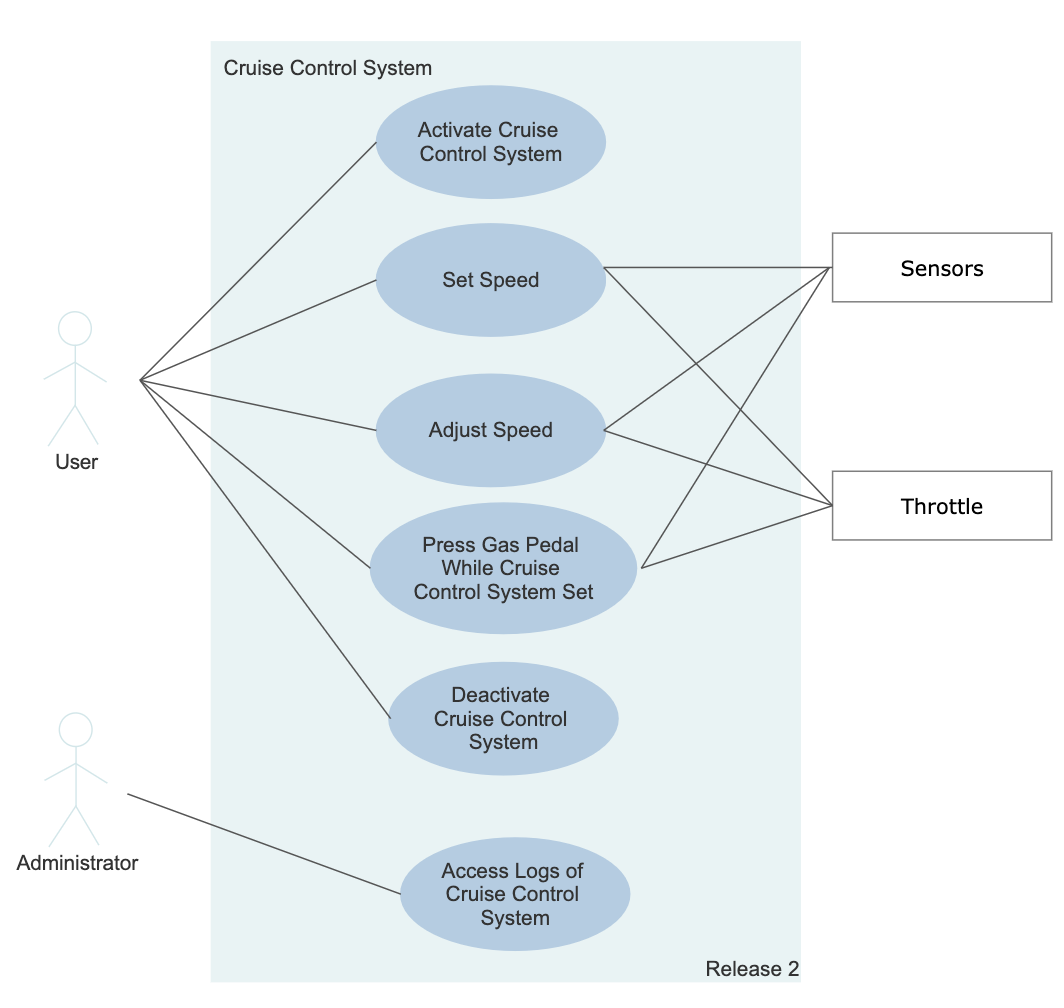
\includegraphics[width=0.9\textwidth]{images/ccUseCaseUML.png}
		\caption{Sample UML diagram for cruise control system use cases.}
		\label{fig:ccUML1}
	\end{figure}

It should be mentioned that there are two similar sounding states that need to be clarified:
\begin{itemize}
	\item Activated
		\begin{itemize}
			\item Granted the vehicle is on, the cruise control system is also now waiting for the speed to be set by the user.
		\end{itemize}
	\item Set/Unset
		\begin{itemize}
			\item Given that the cruise control system has been \textbf{activated}, the user has requested for the speed to be maintained at its current speed.
			\item Given that the cruise control system has been \textbf{activated} and the cruise control system is in the \textbf{set} state, the user can either press the brake or press a button to unset the speed and revert back to the \textbf{activated} state.
		\end{itemize}
\end{itemize}

\begin{enumerate}
	\item 	Use Case 1:\par
			Primary Actor: User\par
			Description: User activates the cruise control system\par
			Outcome: The cruise control system is now activated\par
			Basic Flow:
		\begin{enumerate}
			\item Given that the vehicle is on, the user requests an activation of the cruise control system.
			\item Cruise control system activates.
			\item The cruise control system provides a visual feedback that it has been activated.
		\end{enumerate}
	\item 	Use Case 2: \par
			Primary Actor: User \par
			Description: User sets the speed\par
			Outcome: The speed of the cruise control System is set to a specific speed\par
			Basic Flow:
		\begin{enumerate}
			\item Given that the vehicle is on and the cruise control system is in the activated state, the system requests values from sensors.
			\item Sensors provide values for approval to set cruise control system at current speed.
			\item Cruise control system requests the Engine Management System (EMS) set the speed at current position.
			\item EMS Speed (Throttle) is set at current speed.
			\item Cruise control system provides visual feedback to the user that the cruise control is set and working.
			\item Sensors provide the changing environmental information to the cruise control unit (such as speed, request for increase/decrease speed, and brake).
			\item Cruise control system detects the changes from the sensors and request adjusting speed or deactivating Cruise Control system accordingly.
			\item Speed (Throttle) position is continuously set to new values to ensure that the speed remains constant.
			\item Speed is continuously reported to the cruise control system.
		\end{enumerate}
	\item 	Use Case 3: \par
			Primary Actor: User \par
			Description: User increases speed\par
			Outcome: The speed of the Cruise Control System is increased\par
			Basic Flow:
		\begin{enumerate}
			\item If the cruise control system is in the set state, the user requests an increase of cruise control system speed.
			\item Cruise control system provides visual feedback that the system will alter the speed of the vehicle.
			\item Cruise control system slowly increases the speed of the vehicle to match that of the request.
			\item When the desired speed is reached, the cruise control system will provide visual feedback that the adjustment has been completed.
		\end{enumerate}
	\item 	Use Case 4: \par
			Primary Actor: User \par
			Description: User decreases speed\par
			Outcome: The speed of the Cruise Control System is decreased\par
			Basic Flow:
		\begin{enumerate}
			\item If the cruise control system is in the set state, the user requests a decrease of cruise control system speed.
			\item Cruise control system provides visual feedback that the system will alter the speed of the vehicle.
			\item Cruise control system slowly decreases the speed of the vehicle to match that of the request.
			\item When the desired speed is reached, the cruise control system will provide visual feedback that the adjustment has been completed.
		\end{enumerate}
	\item 	Use Case 5: \par
			Primary Actor: User \par
			Description: User presses gas pedal while the cruise control system is set\par
			Outcome: The speed of the vehicle increases while the gas remains pressed. When the gas is released, the speed will return to the speed of the Cruise Control System\par
			Basic Flow:
		\begin{enumerate}
			\item If the cruise control system is in the set state, the user presses on the gas pedal.
			\item In the event that the vehicle accelerates, the cruise control system will continually request the EMS to be set to the previously specified speed.
			\item Speed will be continuously reported to the cruise control system.
			\item After the user releases the gas pedal and the vehicle stops accelerating, the cruise control system will request for the EMS to be set to the previous specified speed.
			\item The vehicle will naturally decelerate nearing the old set speed, and once reached, the cruise control system will resume with the set speed.
		\end{enumerate}
	\item 	Use Case 6: \par
			Primary Actor: User \par
			Description: User applies brake while the cruise control system is set \par
			Outcome: The speed of the vehicle decreases while the brake remains applied. When the brake is released, the speed will return to the speed of the Cruise Control System\par
			Basic Flow:
		\begin{enumerate}
			\item If the cruise control system is in the set state, the user presses on the brake.
			\item In the event that the vehicle decelerates, the cruise control system will continually request the EMS to be set to the previously specified speed.
			\item Speed will be continuously reported to the cruise control system.
			\item After the user releases the brake and the vehicle stops decelerating, the cruise control system will request for the EMS to be set to the previous specified speed.
			\item The vehicle will naturally accelerate nearing the old set speed, and once reached, the cruise control system will resume with the set speed.
		\end{enumerate}
	\item 	Use Case 7:\par
			Primary Actor: User \par
			Description:  User deactivates cruise control system\par
			Outcome: The Cruise Control System is now deactivated\par
			Basic Flow:
		\begin{enumerate}
			\item If the cruise control system is activated, the user requests a deactivation of the cruise control system.
			\item Cruise control system deactivates.
			\item Cruise control system provides visual feedback that it has been deactivated.
		\end{enumerate}
	\item 	Use Case 8: \par
			Primary Actor: Administrator\par
			Description: Administrator accesses logs of cruise control system\par
			Outcome: The administrator is given access to the log of the Cruise Control System\par
			Basic Flow:
		\begin{enumerate}
			\item With the vehicle turned on and the cruise control activated, an administrator will have to use a proprietary physical hardware key in order to gain root access.
			\item Once access has been granted, the administrator can download the logs to an external storage device through a USB port.
			\item Once downloaded, the administrator must log out using the same proprietary physical hardware key.
		\end{enumerate}
\end{enumerate}

\subsection{UML Class-Based Modeling}
\begin{enumerate}
	\item See Figure ~\ref{fig:classUML} for the class-based modeling for the cruise control system.
		\begin{figure}[H]
			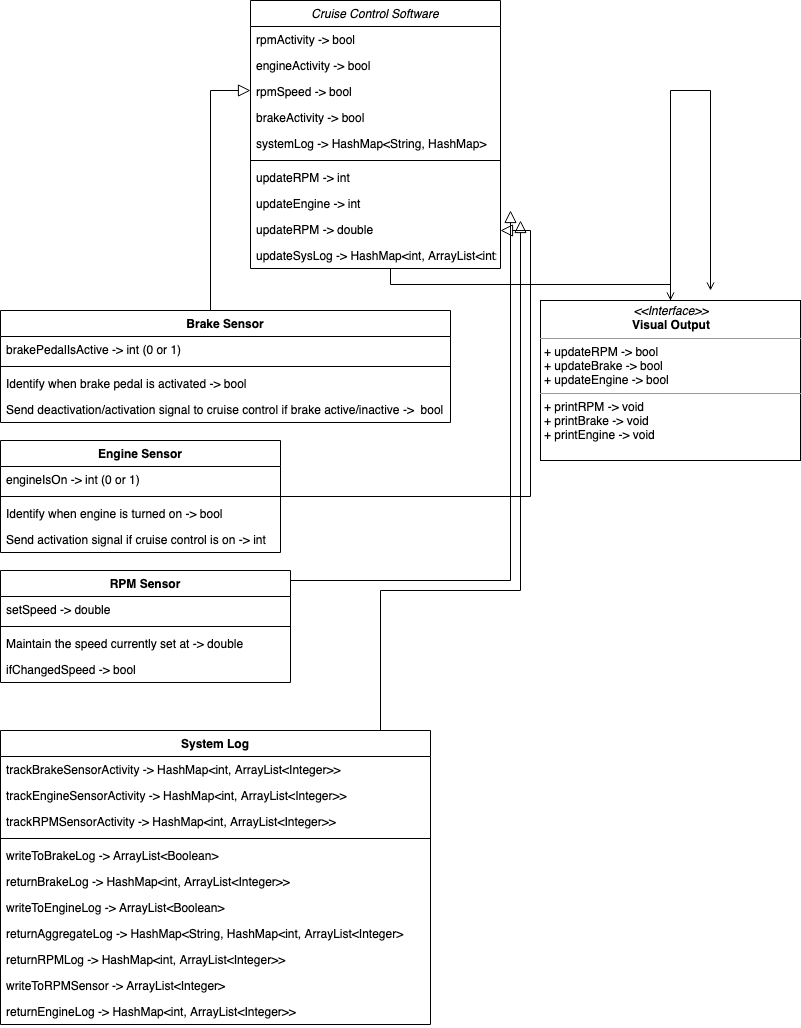
\includegraphics[width=0.9\textwidth]{images/classUML.png}
			\caption{Sample UML class-based model for the cruise control system.}
			\label{fig:classUML}
		\end{figure}
\end{enumerate}

\subsection{UML CRC Model Index Card}
\begin{enumerate}
	\item See Figure ~\ref{fig:indexUML} for the CRC Model Index Cards for the cruise control system.
		\begin{figure}[H]
			\begin{subfigure}{.3\textwidth}
				\centering
				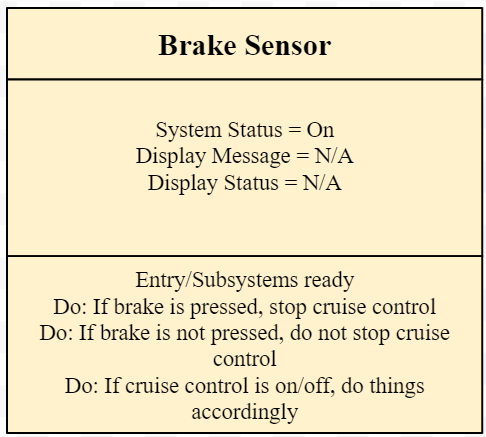
\includegraphics[width=.8\linewidth]{images/brakesensorindex.PNG}
				\label{fig:sub1}
			\end{subfigure}
			\begin{subfigure}{.3\textwidth}
				\centering
				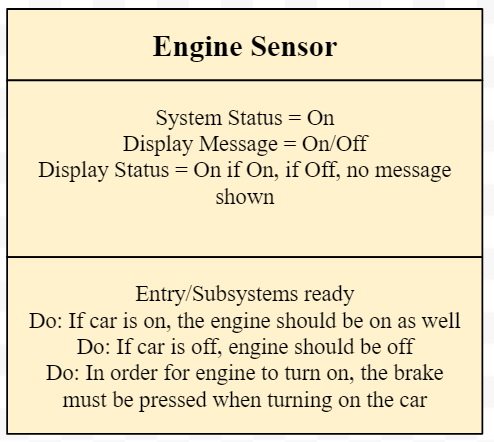
\includegraphics[width=.8\linewidth]{images/enginesensorindex.PNG}
				\label{fig:sub2}
			\end{subfigure}
			\begin{subfigure}{.3\textwidth}
				\centering
				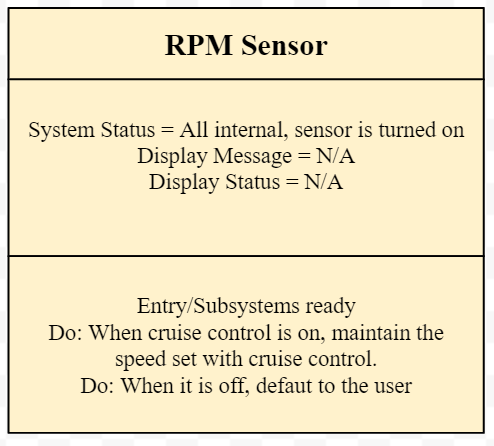
\includegraphics[width=.8\linewidth]{images/rpmsensorindex.PNG}
				\label{fig:sub3}
			\end{subfigure}
			\center
			\begin{subfigure}{.3\textwidth}
				\centering
				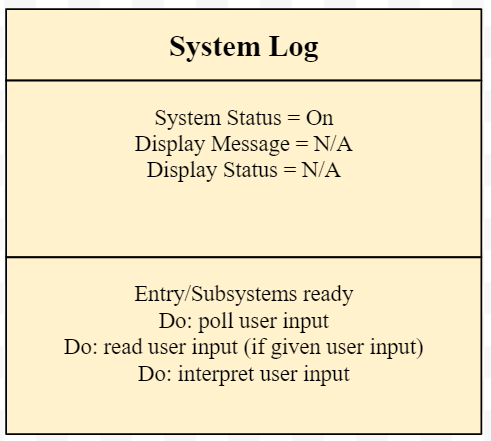
\includegraphics[width=.8\linewidth]{images/systemlogindex.PNG}
				\label{fig:sub3}
			\end{subfigure}
			\begin{subfigure}{.3\textwidth}
				\centering
				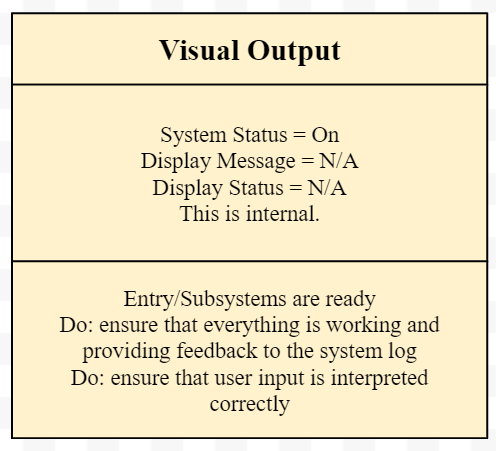
\includegraphics[width=.8\linewidth]{images/visualoutputindex.PNG}
				\label{fig:sub3}
			\end{subfigure}
			\caption{Sample UML CRC model index cards for the cruise control system.}
			\label{fig:indexUML}
		\end{figure}
\end{enumerate}

\subsection{UML Activity Diagram}
\begin{enumerate}
	\item See Figure ~\ref{fig:activityUML} for the activity diagram of the cruise control system.
		\begin{figure}[H]
			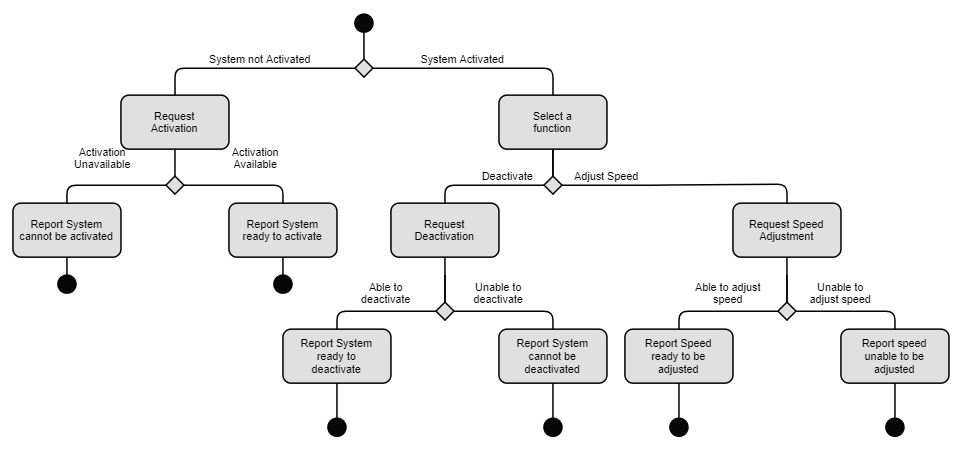
\includegraphics[width=0.9\textwidth]{images/activityUML.jpg}
			\caption{Sample UML activity diagram for the cruise control system.}
			\label{fig:activityUML}
		\end{figure} 
\end{enumerate}

\subsection{UML Sequence Diagram}
\begin{enumerate}
	\item See Figure ~\ref{fig:ccActivation} for sequence diagram of the activation of the cruise control system.
		\begin{figure}[H]
			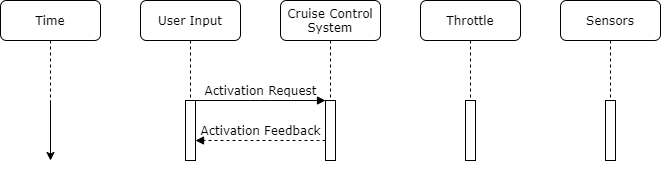
\includegraphics[width=0.9\textwidth]{images/activation.png}
			\caption{Sequence UML digram for activation of the cruise control system.}
			\label{fig:ccActivation}
		\end{figure}
	\item See Figure ~\ref{fig:ccSet} for sequence diagram of cruise control system setting speed.
		\begin{figure}[H]
			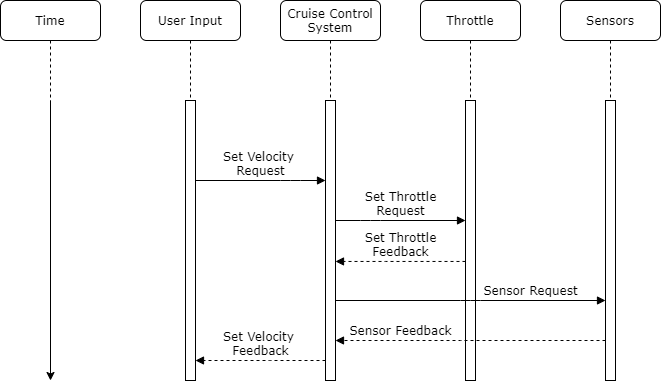
\includegraphics[width=0.9\textwidth]{images/set.png}
			\caption{Sequence UML diagram for the cruise control system setting speed.}
			\label{fig:ccSet}
		\end{figure}
		\newpage
	\item See Figure ~\ref{fig:ccAdjust} for sequence diagram of cruise control system adjusting speed.
		\begin{figure}[H]
			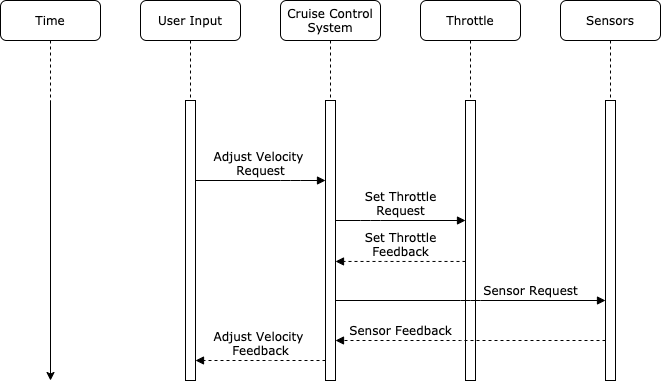
\includegraphics[width=0.9\textwidth]{images/adjustSequence.png}
			\caption{Sequence UML diagram for the cruise control system adjusting speed.}
			\label{fig:ccAdjust}
		\end{figure}
		\newpage
	\item See Figure ~\ref{fig:ccGas} for sequence diagram of the cruise control system being suspended when the user presses the gas pedal.
		\begin{figure}[H]
			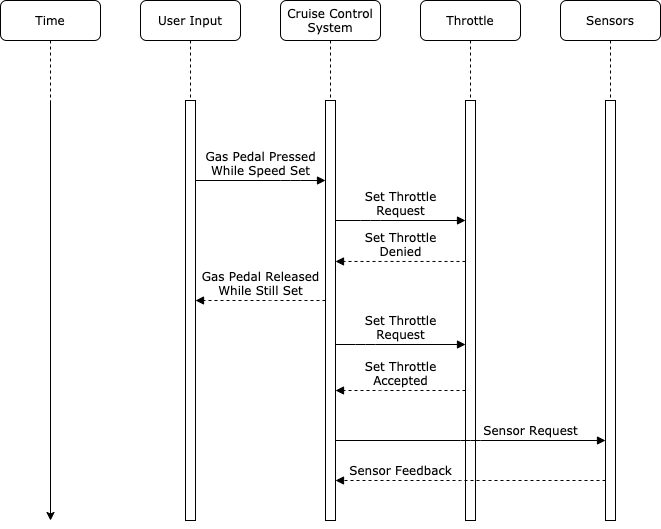
\includegraphics[width=0.9\textwidth]{images/gasPedalPressedSequence.png}
			\caption{Sequence UML diagram for the cruise control system suspending during gas pedal being pressed.}
			\label{fig:ccGas}
		\end{figure}
		\newpage
	\item See Figure ~\ref{fig:ccDeactivate} for sequence diagram of the cruise control system being deactivated.
		\begin{figure}[H]
			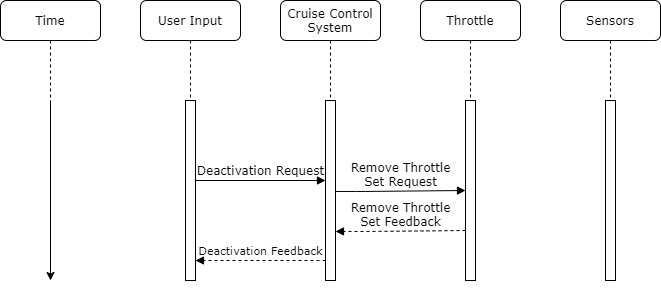
\includegraphics[width=0.9\textwidth]{images/deactivation.png}
			\caption{Sequence UML diagram for the cruise control system being deactivated.}
			\label{fig:ccDeactivate}
		\end{figure}
		\newpage
	\item See Figure ~\ref{fig:ccAdmin} for sequence diagram of the administrator accessing the cruise control system logs.
		\begin{figure}[H]
			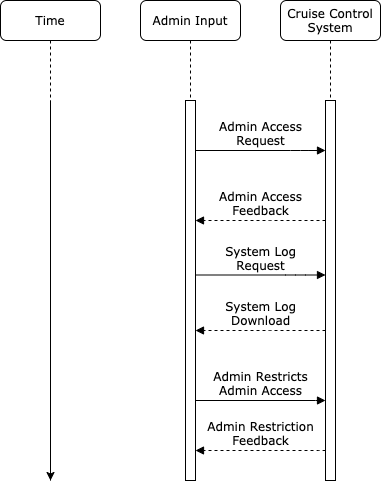
\includegraphics[width=0.9\textwidth]{images/sequenceAdmin.png}
			\caption{Sequence UML diagram for the administrator accessing cruise control system logs.}
			\label{fig:ccAdmin}
		\end{figure}
\end{enumerate}

\newpage
\subsection{UML State Diagram}
\begin{enumerate}
	\item See Figure ~\ref{fig:stateUML} for the state diagram of the cruise control system.
			\begin{figure}[H]
				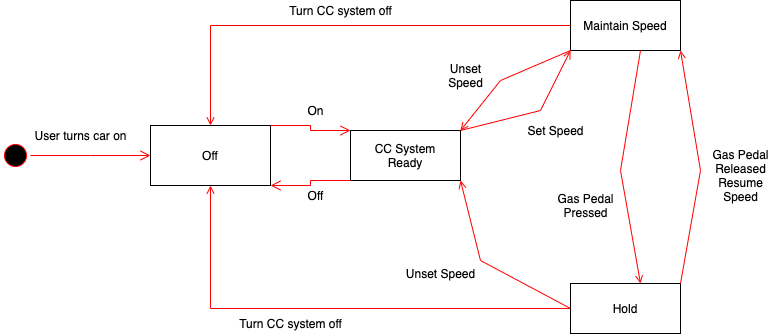
\includegraphics[width=0.9\textwidth]{images/stateUML.png}
				\caption{Sample UML state diagram for the cruise control system.}
				\label{fig:stateUML}
			\end{figure}
\end{enumerate}

\newpage
\section{Software Architecture}

\subsection{Architecture Style} 
We decided to implement our Cruise Control System by using Object Oriented Programming.
\begin{enumerate} 
	\item We chose this architecture style because it will allow us to represent the different aspects of the cruise control system as different objects. For example, we will be able to represent the engine, the brake, the throttle, the sensors, and the log as different objects. These objects will have different attributes which will allow the program to closely resemble the real world. The brake object will contain a boolean that determines if the brake is being pressed or not. It will also have a function that will decrease the current speed of the vehicle. The sensors will have variables that determine if the current speed is less than, greater than, or equal to the desired cruising speed. The throttle will contain a boolean that determines if the user is trying to manually increase the speed of the vehicle. It will also have a function that will increase the speed of the car. The engine object will contain a boolean that determines if the vehicle is on or off. The log will be a tuple of a time stamp and a string. Whenever any action is taken by the driver or the cruise control system, it will be added to the log. All of these objects will be used as components of a larger Cruise Control System object.
	\item Using object-oriented design will limit the number of programming languages that we would be able to use. Using object-oriented programming can result in more resources being used because the programs can become very large. It is also difficult to determine all of the classes that will be necessary in order to properly implement the Cruise Control System at the beginning of the project.
	\item We also considered implementing our Cruise Control System with call and return architecture. This architecture design would have allowed us to split the main program into subprograms. It would have been easier to build upon the program by adding more subprograms. It would have also been able to set a hierarchy for different programs if we used the main program/subprogram style of this architecture.
	\item We opted not to use a call and return architecture because this architectural design often does not adequately support the data structures which would be important for the implementation of the Cruise Control System. Furthermore, due to a large number of subprograms, it may have become difficult to navigate and manage. 
	\item We did not consider the following architectures:
		\begin{enumerate} 
			\item The components of a system encapsulate data and the operations that must be applied to manipulate the data. Communication and coordination between components are accomplished via message passing. 
			\item Pros: It models the real world very well. With OOP, programs are easy to understand and maintain. OOP offers code re-usability. Already created classes can be reused without having to write them again.OOP facilitates the quick development of programs where parallel development of classes is possible.With OOP, programs are easier to test, manage and debug.
			\item Cons: With OOP, classes sometimes tend to be over-generalized. The relations among classes become superficial at times. The OOP design is tricky and requires appropriate knowledge. Also, one needs to do proper planning and design for OOP programming. To program with OOP, the programmer needs proper skills such as that of design, programming and thinking in terms of objects and classes etc.
		\end{enumerate} 
\end{enumerate}

\subsection{Components} 
A software component is an architectural entity that encapsulates a subset of the system’s functionality and/or data. A set of components will perform a function that is required by a system. This restricts access to that subset via an explicitly defined interface. The components of a software system are the following (but not limited to):
\begin{enumerate} 
	\item Network and Internet services
	\item Hardware level of operating system
	\item Logical level of operating system
	\item Graphics engine
	\item User interface
	\item System services
	\item Command shell
	\item System utilities 
\end{enumerate} 
Regarding cruise control specifically, the main component of our cruise control is the engine management system. In order to do this, the cruise control will receive data from the sensor components in which it relays data from the components of the car (take for example, the brake and the sensors). \par
Components and connectors are used to accomplish a system's goal. This is expressed through an architectural configuration. More precisely, an architectural configuration is an association between components and connectors of software architecture. A connector is not equivalent to a component as components provide application-specific functionality while connectors provide application-independent interaction mechanisms.\par
Connectors are between the sensors to deliver the data to the cruise control module. This processes the data to determine the speed of the car. The connectors between the cruise control and the engine management system will continually deliver this data to each other.\par
A software constraint defines how components can be integrated to form the system. A software constraint is a restriction on the degree of freedom you have in providing a solution. Constraints are effectively global requirements, such as limited development resources or a decision by senior management that restricts the way you develop a system.\par
The information that is shared between the sensor components to the signal that the engine has been started must be delivered very quickly before cruise control can be turned on. The activation and deactivation of cruise control must be done in a specific time constraint. These are all constraints of the system.\par

\subsection{Control Management} 
	\begin{figure}[H]
		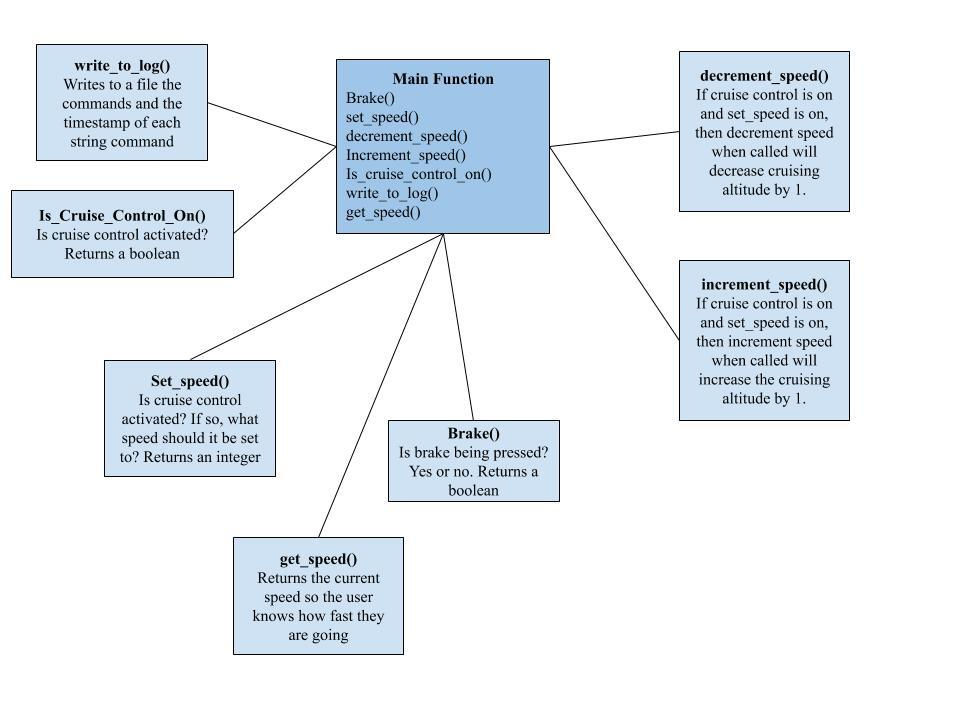
\includegraphics[width=0.9\textwidth]{images/Control_Management_Diagram.jpg}
		\caption{Control management diagram}
		\label{fig:control_mgmt_diagram}
	\end{figure}\par
	We are going to have a main function that will have calls to the functions listed above as you can see: write_to_log(), Is_Cruise_Control_On(), Set_speed(), get_speed(), Brake(), increment_speed(), and decrement_speed(). These functions are essentially what are going to control our cruise control module. Brake will be a boolean as it is either true that the brake is being pressed or false if it is not being pressed. If cruise control is on and there is a set speed that is greater than 25 (which is the only way that cruise control can be activated in the first place), then if the brake function goes from false to true, then we shut off the cruise control entirely. \par 
	This is similarly listed out in the diagram as shown. All of our functions interact with our main function which is essentially the driver of our cruise control program. 


\subsection{Data Architecture} 
In terms of data architecture, considering that the project is going to be programmed in an object-oriented language such as Java, having the data schema represented in the same programming paradigm streamlines the technical thought process behind the project. Having a data schema known for reliability is imperative for a mission-critical piece of software like cruise control.\par
Due to the use of Java, the general paradigm of the data architecture is object-oriented.  Communication between the components is done via passing information as parameters to functional components such as methods and classes. Cruise control software requires information to be readily available to make critical decisions. An architecture based on passing information as parameters allows us to continually pass around data within the system, making data access trivially fast and facilitates quick decisions and computations that can mitigate the risk of fatal injury or things spiraling out of control.\par
To optimally implement this structure, we would need to define several functional components that each handles its own individual task and can be called as a function call to perform its individual task quickly. So, the cruise control system can have its own functional component for controlling the speed, controlling the brake, and sending visual and audio information to the user to inform about cruise control status such as whether it is on or off. The data components would always be available for use for functional components (such as program methods) in the cruise control software. This is because the functional components will need to repeatedly query the data components to accurately compute what speed is necessary, whether a brake is needed, and whether the user has requested for the system to turn on or off.\par
 
\newpage
\subsection{Architectural Designs} 
\begin{enumerate}
	\item See Figure ~\ref{fig:context} for the architecture context diagram in which the external entities that the software interacts with are defined. Some include other systems, devices, and actors.
		\begin{figure}[H]
			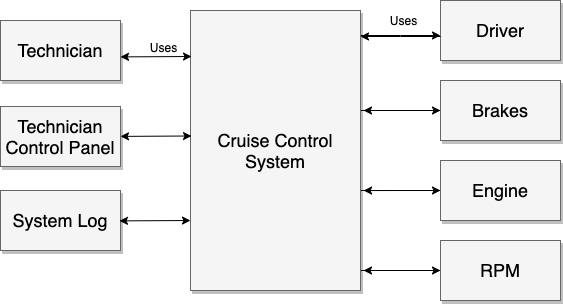
\includegraphics[width=0.9\textwidth]{images/Architectural_Context_Diagram.png}
			\caption{context diagram}
			\label{fig:context}
		\end{figure}
		\newpage
	\item See Figure ~\ref{fig:set} for the cruise control archetype. The archetype is an abstraction that represent an element of the cruise control system behavior.
				\begin{figure}[H]
					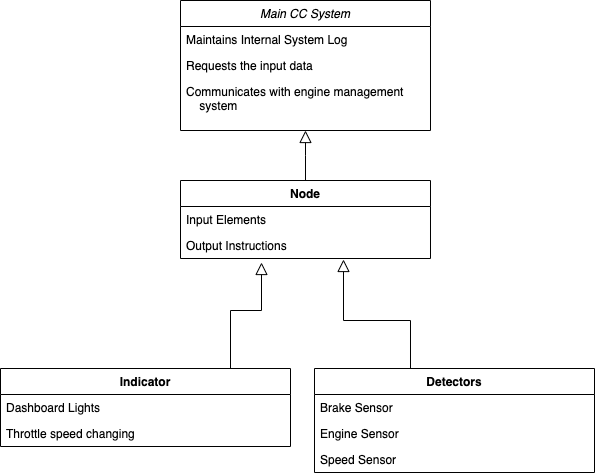
\includegraphics[width=0.9\textwidth]{images/classMapCS347_set.png}
					\caption{Cruise Control System Archetypes}
					\label{fig:set}
				\end{figure}
				\newpage
	\item See Figure ~\ref{fig:top} for the cruise control top-Level component in which the archetype is further defined for help with implementation.
		\begin{figure}[H]
			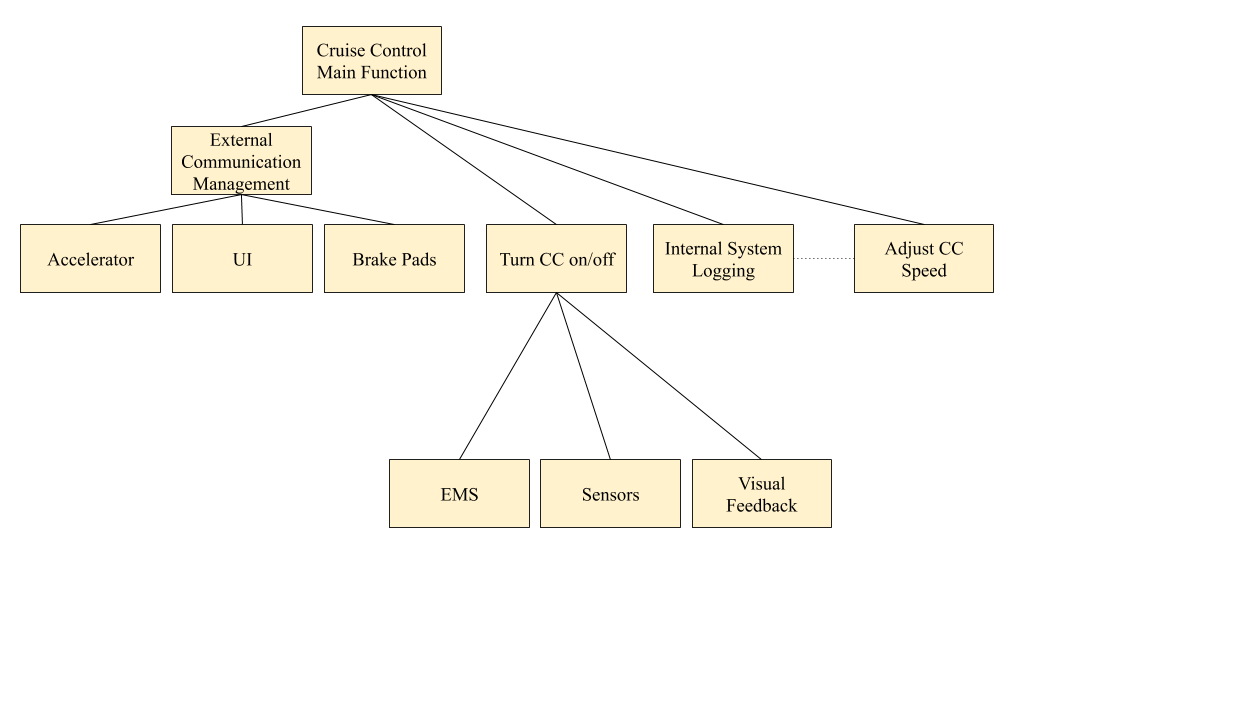
\includegraphics[width=0.9\textwidth]{images/Architecture_Top.png}
			\caption{Top-level component}
			\label{fig:top}
		\end{figure}
	\item See Figure ~\ref{fig:refined} for the refined component architecture. This is a more refined version of the top-level component to help with implementation as well.
		\begin{figure}[H]
			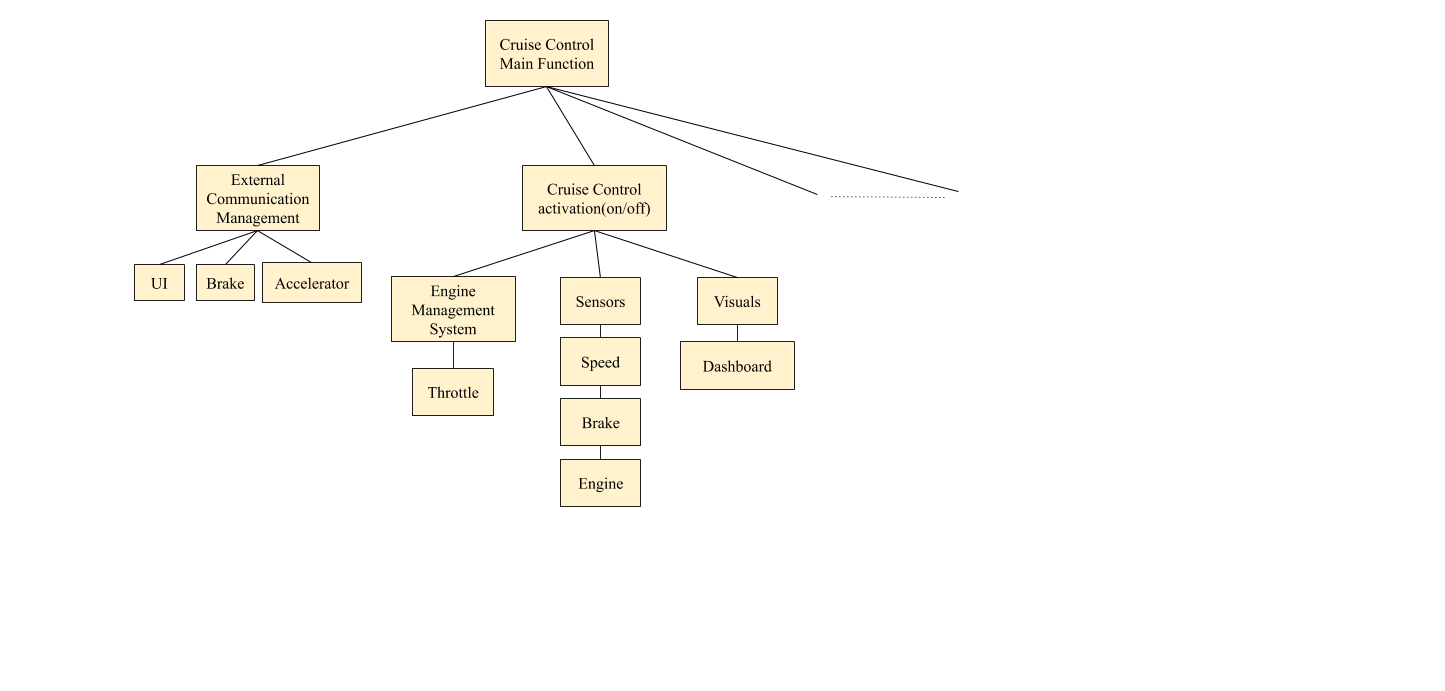
\includegraphics[width=\textwidth]{images/Refined_Components.png}
			\caption{Refined component}
			\label{fig:refined}
		\end{figure}
\end{enumerate}

\subsection{Issues}
\begin{enumerate} 
	\item Hamzah: The data architecture has not been thoroughly defined. Work through the data architecture and define how exactly the cruise control software will store the data using MongoDB in an object-oriented + call and return architecture. Review section 5.3.\textbf{Resolved: 4/17/2020}
	\item Connie: work with Hamzah to identify how control interacts with the Data Architecture and the drawbacks of Object-Oriented design and call and return architectures. Review section 5.3.\textbf{Resolved: 4/17/2020}
	\item Eric: Make security contingencies in case of data leak/ security issues. There needs to be a consideration of the ramifications that using a database like MongoDB can have security wise due to the fact that it is cloud based. Perhaps creating our own local database that behaves similarly to a black box would be the most secure option. Review section 5.4.\textbf{Resolved: 4/16/2020}
	\item Mike: Consider any architectural alternatives to the current design to ensure that the best implementation is chosen. Review section 5.5.\textbf{Resolved: 4/18/2020}
	\item Mike: In section 5.1, what does it mean where it says “the log will be an array”?\par
			As each command for cruise control comes in, we will append it to a file as opposed to maintaining an array. This is not to say the log will not be treated like an object as each message will be a tuple of a time stamp and a string which will be appended to the log file. \textbf{Resolved: 5/4/2020}
	\item Mike: Do we want to keep in section 5.2 the general definition of components in software?\par
			Yes, we do want to keep it as it helps guide understanding of how we will be using components. \textbf{Resolved: 5/4/2020}
	\item Connie: In section 5.3, we should add a write_to_log() function.\par
			We added another function to our Control Management Diagram in Section 5.3 that would write each command to the log. \textbf{Resolved: 5/4/2020}
	\item Connie: In section 5.3, we should add some accessor functions in our control management diagram.\par
			We added more functions to our Control Management Diagram in Section 5.3 that act as accessor methods. For example, we added: getSpeed(), and isCruiseControlOn() that return the current state of the vehicle. \textbf{Resolved: 5/4/2020}
	\item Eric: In section 5.4, did we specify the specific programming language we will be using?\par
			We were deciding between implementing the Cruise Control System in Java or C++. We ultimately decided to use Java because the group as a whole feels more comfortable programming in this language. \textbf{Resolved: 5/4/2020}
	\item Eric: In section 5.4, why are we using a database for local cruise control?\par
			Removal of the database as it will not be scalable so there is no reason to keep it. More so, since this is a local prototype and there is not a reason to connect the database. In order to store information, we have other means for it. It also leaves room for hackers to tamper with the software. \textbf{Resolved: 5/4/2020}
	\item Hamzah: In section 5.4, there is a grammatical error in the first sentence of the last paragraph.\par
			This grammatical error was corrected. \textbf{Resolved: 5/4/2020}
	\item Hamzah: In section 5.6, we need to specify where the issues were in section 5.\par
			The issues that were resolved in section 5.6 were updated to include the section where the issue was found. \textbf{Resolved: 5/4/2020}
	\item Eric: The formatting of the charts in section 4.5 is off.\par
			The diagrams in section 4.5 were reformatted to correct mistakes that were made when uploading the diagram to the document. This will make comprehension of the diagrams much easier. \textbf{Resolved: 5/4/2020}
	\item Connie: There is a spelling error in section 4.1.\par
			This spelling error was corrected. \textbf{Resolved: 5/4/2020}
\end{enumerate}

\end{document}

